% !TEX program = xelatex

% Nejlepší zážitek zaručí:
%
% TeX distribuce: texlive-full
%
% Editor:
%   VS Code s doplňky
%       * LaTeX Workshop
%       * LaTeX Utilities
%       * Gnuplot
%
% Další závislosti:
%   latexmk
%   bibtex
%   gnuplot


% Jak používat:
% Zkompilovat: make
% Gnuplot: make gnuplot
% Vyčistit: make clean


% Základní balíčky
\documentclass[10pt,a4paper]{article}
\usepackage[utf8]{inputenc}
\usepackage[czech]{babel}
\usepackage{graphicx}
\usepackage{lmodern}
\usepackage{amsmath}
\usepackage[top = 2cm, bottom = 2cm, left = 2cm, right = 2cm]{geometry}

% Pro titulní stránku
\usepackage{titlesec}
\usepackage{setspace}
\usepackage{framed}
\usepackage{array}

% Vlastní balíčky 
\usepackage{gnuplottex}
\usepackage{epstopdf}
\usepackage{csvsimple}


\newcommand{\titjmeno}{Michal Grňo}
\newcommand{\titobor}{FOF}


\newcommand{\titcislo}{A7}
\newcommand{\titnazev}{Pozitronová emisní tomografie}
\newcommand{\titmereni}{7. 10. 2019}
\newcommand{\titodevzdani}{20. 10. 2019}


\begin{document}


\thispagestyle{empty}
\newgeometry{top = 2.5cm, bottom = 0cm, left = 2.5cm, right = 3cm}

{%T tomto je uzavřena celá titulka
%Tloušťka rámečku
\setlength{\fboxrule}{1.5pt}

\noindent
\framebox{
\begin{minipage}{\textwidth}
\setlength{\parindent}{17.62482 pt}
\phantom{d}

\begin{minipage}{0.6\textwidth}
{
\Large Kabinet výuky obecné fyziky, UK MFF\\
}
\vspace*{0.2cm}

{
\bfseries
\huge Fyzikální praktikum %ČÍSLO
}
\end{minipage}
\begin{minipage}{0.4\textwidth}
\begin{center}
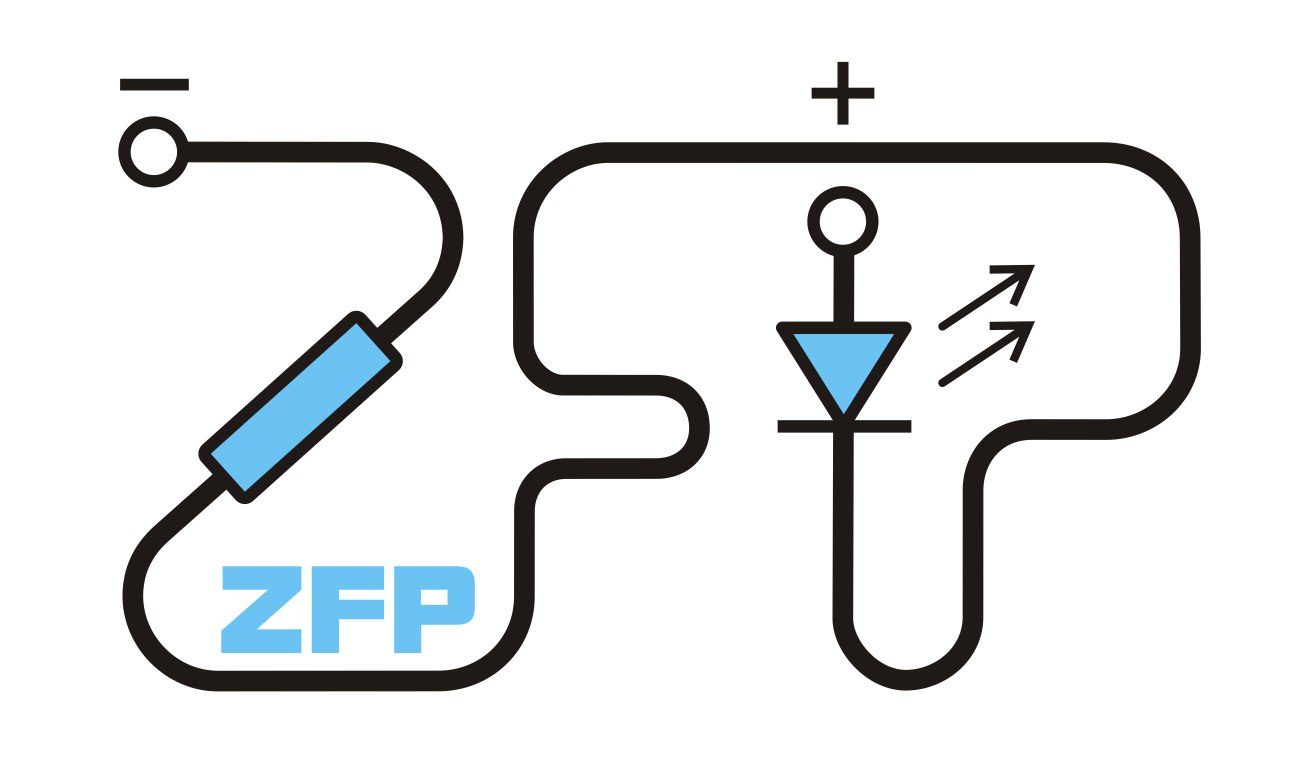
\includegraphics[width=4.5cm]{ZFP.jpg}
\end{center}
\end{minipage}\\\\

%\vspace*{0.5cm}

{
\setstretch{1.5}
\Large
\noindent
Úloha č. \titcislo

\noindent
Název úlohy: \titnazev

\noindent
Jméno: \titjmeno
\hspace*{\fill}
Obor: \titobor

\noindent
Datum měření: \titmereni
\hspace*{\fill}
Datum odevzdání: \titodevzdani

\phantom{d}
}
\end{minipage}
}
%Konec horního rámečku

{
\phantom{d}

\Large
Připomínky opravujícího:\\
\vspace*{6.75cm}
}

\newcommand{\linka}{\noalign{\hrule height 1pt}}
\newcommand{\linkadva}{\noalign{\hrule height 1.5pt}}
\setlength\extrarowheight{9.5pt}
\Large
\noindent
\begin{tabular}{!{\vrule width 1.5pt} l !{\vrule width 1pt} c !{\vrule width 1pt} c !{\vrule width 1.5pt}}
\linkadva
   & Možný počet bodů & Udělený počet bodů \\\linkadva
  Práce při měření & 0-3 &  \\\linka
  Teoretická část & 0-2 &  \\\linka
  Výsledky a zpracování měření & 0-9 &  \\\linka
  Diskuse výsledků & 0-4 &  \\\linka
  Závěr & 0-1 &  \\\linka
  Použitá literatura & 0-1 &  \\\linkadva
  \hspace*{\fill} \textbf{Celkem} \hspace*{\fill}& max. 20 &  \\
\linkadva
\end{tabular}
\phantom{d}

Posuzoval: \hspace*{\fill}dne:~~~~~~~~~~~~~~~~~

}%Konec uzavření titulky
\newpage
\newgeometry{top = 2cm, bottom = 2cm, left = 2cm, right = 2cm}
\setcounter{page}{1}

\section{Pracovní úkoly}
\begin{enumerate}
    \item Poté, co vyučující umístí silnější zářič ${}^{22}$Na do stojánku, změřte úhlové rozdělení koincidencí v oblasti úhlů potřebné pro nalezení polohy zářiče, doba měření 20s. Vysvětlete tvar naměřeného úhlového rozdělení, získané poznatky využijte při domácím zpracování.

    \item Změřte četnost koincidencí pro úhly $\phi$ = 60°, 90°, 120° bez plechu a 120° s Pb plechem mezi detektory, doba měření 100s. Vysvětlete pozorované četnosti.
    
    \item Poté, co vyučující přidá do krabičky druhý zářič, změřte úhlové rozdělení koincidencí s krokem 5°.
    
    \item Zvolte aspoň 2 další vhodné úhly otočení krabičky $\psi$ a opakujte měření 3).
    
    \item Narýsujte přímky spojující detektory do obrázku připraveného u úlohy a odečtěte polohu průsečíku - polohu zářiče vůči krabičce. Pozn.: Při volbě otočení krabičky $\psi$ se můžete řídit polohou už zakreslených průsečíků.
    
    \item Vzdálenost detektoru od zářiče zakresleného na obrázku porovnejte s měřením skutečné vzdálenosti.
    
    \item Polohy zářičů vůči krabičce určujte pomocí vztahů a metod popsaných v návodu. Podle výsledků zpracování nakreslete obrázky analogické k obrázkům narýsoaným během praktika. Chyby polohy zářičů určete graficky
\end{enumerate}


\section{Teoretická část}
Teorie\cite{DUMMY:1}
\begin{equation*}
    A = 4
    \label{A}
\end{equation*}

\begin{figure}[h]
    \centering
    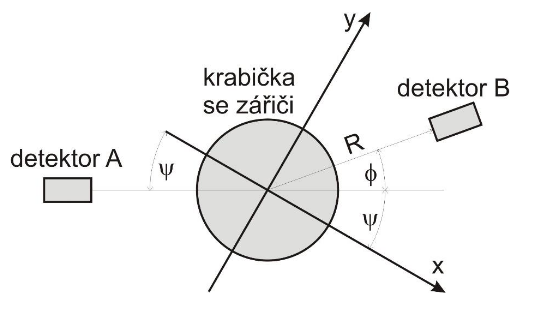
\includegraphics[width=10cm]{schema.png}
    \caption{Schéma koincidenčního měření, převzato z [1].}
\end{figure}


\section{Výsledky měření}
Naměřil jsem 3.


\begin{table}[h!]
    \centering
    \begin{tabular}{r|r|r}
        % Hlavička
        \bfseries $\psi$ &
        \bfseries $\varphi$ &
        \bfseries $\Delta\varphi$

        % Soubor
        \csvreader[ head to column names ]{fits1.csv.tmp}{}
        {
            \csviffirstrow{\\\hline}{\\} \psival\ & \phival & \phierr
        }
    \end{tabular}

    \caption{Úhly získané regresí}
    \label{tab-fity-1vz}
\end{table}


\begin{table}[h!]
    \centering
    \begin{tabular}{r|r|r|r|r}
        % Hlavička
        \bfseries $\psi$ &
        \bfseries $\varphi_1$ &
        \bfseries $\Delta\varphi_1$ &
        \bfseries $\varphi_2$ &
        \bfseries $\Delta\varphi_2$

        % Soubor
        \csvreader[ head to column names ]{fits3.csv.tmp}{}
        {
            \csviffirstrow{\\\hline}{\\}
            \psival\ &
            \phiA & \phiAerr &
            \phiB & \phiBerr
        }
    \end{tabular}
    
    \caption{Úhly získané regresí}
    \label{tab-fity-1vz}
\end{table}



\begin{figure}[p]
    \centering
    \begin{gnuplot}[terminal=epslatex,terminaloptions=color]

        set xlabel "$\\varphi$ [\°]"
        set ylabel "N"
        load 'lines.cfg'
        set macros
        set key left top

        nd(A, x0, sigma, x) = A * exp(-(x-x0)**2/2./sigma**2)


        colselector(phi) = \
            '( $1 > 180 ? $1 - 360 : $1 ):($3 == '.phi.' ? $2 : 1/0)'
        
        set1 = colselector(0)
        set2 = colselector(30)
        set3 = colselector(60)
        set4 = colselector(90)

        A1 = A2 = A3 = A4 = 400
        mean1 = mean2 = mean3 = mean4 = 1
        sigma1 = sigma2 = sigma3 = sigma4 = 5


        f1(x) = nd(A1, mean1, sigma1, x)
        f2(x) = nd(A2, mean2, sigma2, x)
        f3(x) = nd(A3, mean3, sigma3, x)
        f4(x) = nd(A4, mean4, sigma4, x)


        fit f1(x) 'data1' using @set1 via A1, mean1, sigma1
        fit f2(x) 'data1' using @set2 via A2, mean2, sigma2
        fit f3(x) 'data1' using @set3 via A3, mean3, sigma3
        fit f4(x) 'data1' using @set4 via A4, mean4, sigma4


        set print "fits1.csv.tmp"
        print "psival, phival, phierr"
        print sprintf( "0, %.2f, %.2f", mean1, mean1_err)
        print sprintf("30, %.2f, %.2f", mean2, mean2_err)
        print sprintf("60, %.2f, %.2f", mean3, mean3_err)
        print sprintf("90, %.2f, %.2f", mean4, mean4_err)


        plot \
            'data1' using @set1 notitle lc palette cb 0, \
            f1(x) notitle lc palette cb 0, \
            NaN w lp title "$\\psi$ = 0°" lc palette cb 0, \
            \
            'data1' using @set2 notitle lc palette cb 2, \
            f2(x) notitle lc palette cb 2, \
            NaN w lp title "$\\psi$ = 30°" lc palette cb 2, \
            \
            'data1' using @set3 notitle lc palette cb 3, \
            f3(x) notitle lc palette cb 3, \
            NaN w lp title "$\\psi$ = 60°" lc palette cb 3, \
            \
            'data1' using @set4 notitle lc palette cb 4, \
            f4(x) notitle lc palette cb 4, \
            NaN w lp title "$\\psi$ = 90°" lc palette cb 4

    \end{gnuplot}

    \caption{Naměřené koincidence, jednovzorkový setup}
    \label{graf-1vz}
\end{figure}


\begin{figure}[p]
    \centering
    \begin{gnuplot}[terminal=epslatex,terminaloptions=color]
        
        set xlabel "$\\varphi$ [\°]"
        set ylabel "N"
        set xrange [40:140]
        set yrange [0:80]
        load 'lines.cfg'
        set key left bottom
        set key box vertical width 1 height 1 maxcols 0.3 spacing 1

        plot \
            'data2' using 1:($3 == 0 ? $2 : 1/0) \
                ps 3 lc palette cb 0 title "nestíněný", \
            \
            'data2' using 1:($3 == 1 ? $2 : 1/0) \
                ps 3 lc palette cb 1 title "stíněný" \

    \end{gnuplot}
\end{figure}


\begin{figure}[p]
    \centering
    \begin{gnuplot}[terminal=epslatex,terminaloptions=color]

        set xlabel "$\\varphi$ [\°]"
        set ylabel "N"
        load 'lines.cfg'
        set macros
        set key left top

        arbitrarilyLargeNumber = 1000000000

        nd(A, x0, sigma, x) = A * exp(-(x-x0)**2/2./sigma**2)


        colselector(phi) = \
            '( $1 > 180 ? $1 - 360 : $1 ):($3 == '.phi.' ? $2 : 1/0)'
        
        set1 = colselector(0)
        set2 = colselector(60)
        set3 = colselector(90)

        A1a = A1b = A2a = A2b = A3a = A3b = 400
        mean1a = mean2a = mean3a = mean4a = -20
        mean1b = mean2b = mean3b = mean4b = 20
        sigma1a = sigma2a = sigma3a = sigma4a = 15
        sigma1b = sigma2b = sigma3b = sigma4b = 15
        noise1 = noise2 = noise3 = 1

        f1(x) = noise1 < 0 ? arbitrarilyLargeNumber : \
            nd(A1a, mean1a, sigma1a, x) + nd(A1b, mean1b, sigma1b, x) + noise1

        f2(x) = noise2 < 0 ? arbitrarilyLargeNumber : \
            nd(A2a, mean2a, sigma2a, x) + nd(A2b, mean2b, sigma2b, x) + noise2

        f3(x) = noise3 < 0 ? arbitrarilyLargeNumber : \
            nd(A3a, mean3a, sigma3a, x) + nd(A3b, mean3b, sigma3b, x) + noise3


        fit f1(x) 'data3' using @set1 \
        via A1a, mean1a, sigma1a, A1b, mean1b, sigma1b, noise1

        fit f2(x) 'data3' using @set2 \
        via A2a, mean2a, sigma2a, A2b, mean2b, sigma2b, noise2

        fit f3(x) 'data3' using @set3 \
        via A3a, mean3a, sigma3a, A3b, mean3b, sigma3b, noise3


        set print "fits3.csv.tmp"
        print "psival, phiA, phiAerr, phiB, phiBerr"
        fmt = "%d, %.2f, %.2f, %.2f, %.2f"
        print sprintf(fmt,  0, mean1a, mean1a_err, mean1b, mean1b_err)
        print sprintf(fmt, 60, mean2a, mean2a_err, mean2b, mean2b_err)
        print sprintf(fmt, 90, mean3a, mean3a_err, mean3b, mean3b_err)


        plot \
            'data3' using @set1 notitle lc palette cb 0, \
            f1(x) notitle lc palette cb 0, \
            NaN w lp title "$\\psi$ = 0°" lc palette cb 0, \
            \
            'data3' using @set2 notitle lc palette cb 2, \
            f2(x) notitle lc palette cb 2, \
            NaN w lp title "$\\psi$ = 60°" lc palette cb 2, \
            \
            'data3' using @set3 notitle lc palette cb 3, \
            f3(x) notitle lc palette cb 3, \
            NaN w lp title "$\\psi$ = 90°" lc palette cb 3

    \end{gnuplot}

    \caption{Naměřené koincidence, dvouvzorkový setup}
    \label{graf-2vz}
\end{figure}

\begin{figure}[p]
    \begin{gnuplot}[terminal=epslatex,terminaloptions=color]


        load 'matlib.cfg'
        load 'vzorce.cfg'



        # načti první soubor

        LF_File = 'fits1.csv.tmp'
        LF_Columns = 3
        load 'loadfile.cfg'

        m = sliceArray('LF_Col1','psi',1,0)
        @m
        m = sliceArray('LF_Col2','phi',1,0)
        @m

        do for [i=1:|psi|] { psi[i] = real(psi[i]) }
        do for [i=1:|phi|] { phi[i] = real(phi[i]) }


        # vypočítej průsečíky

        N = nCr(|psi|, 2)
        array xint[N]
        array yint[N]

        i = 1
        do for [j=1:|psi|] {
            do for [k=1:j-1] {
                xint[i] = xintf(psi[j], phi[j], psi[k], phi[k])
                yint[i] = yintf(psi[j], phi[j], psi[k], phi[k])
                i = i + 1
            }
        }


        set xlabel "x"
        set ylabel "y"

        plot sample [i=2:LF_Rows] '+' using (xint[i]):(yint[i]) notitle
    \end{gnuplot}
\end{figure}


\section{Diskuse}
Bylo to špatně protože \eqref{A} 


\section{Závěr}
Bylo to hezké. assadfasd

\section{Literatura}
\bibliography{literatura} 
\bibliographystyle{ieeetr}

 
\end{document}